\documentclass[a4paper, twoside]{report}


%% Language and font encodings
\usepackage[english]{babel}
\usepackage[utf8x]{inputenc}
\usepackage[T1]{fontenc}
\usepackage{amssymb}
\usepackage{tgpagella}
\usepackage{fancyhdr}
%% Sets page size and margins


%% Useful packages
\usepackage{float}
\usepackage{amsmath}
\usepackage{amsthm}
\usepackage{stmaryrd}
\usepackage{graphicx}
\usepackage{mathrsfs}
\usepackage[colorinlistoftodos]{todonotes}
\usepackage[colorlinks=true, allcolors=blue]{hyperref}
\usepackage[classfont=sanserif,langfont=typewriter,funcfont=typewriter]{complexity}
\usepackage{mathtools}
\usepackage{commath}
\usetikzlibrary{patterns}
\usepackage{tikz}
\bibliographystyle{acm}
\usepackage{algpseudocode}
\usepackage[linesnumbered, ruled]{algorithm2e}
\usepackage{enumitem}
\usetikzlibrary{decorations.pathreplacing,angles,quotes,shapes.geometric, arrows, automata, positioning,patterns}
\usepackage{setspace}
\linespread{1.25}

\newtheorem*{theorem*}{Theorem}
\newtheorem{theorem}{Theorem}
\newtheorem{claim}{Claim}
\newtheorem{lemma}{Lemma}
\newtheorem{prop}{Proposition}
\newtheorem{definition}{Definition}
\newtheorem{corollary}{Corollary}[lemma]

\newcommand{\triggers}{\ |\hspace{-1.8mm}\rightarrow}
\newcommand{\followedby}{\ \diamond\hspace{-1.5mm}\rightarrow}
\newcommand{\xtriggers}{\ |\hspace{-1.7mm}\Rightarrow}
\newcommand{\xfollowedby}{\ \diamond\hspace{-1.5mm}\Rightarrow}
\newcommand{\psluntil}{\ensuremath{\textbf{U}}}
\newcommand{\pslnext}{\ensuremath{\textbf{X}}}

\newcommand{\modelspsl}{\models_\textsc{psl}}
\newcommand{\sema}[1]{{\llbracket}#1{\rrbracket}}


%% Sets page size and margins
\usepackage[a4paper,top=3cm,bottom=2cm,left=3cm,right=3cm,marginparwidth=1.75cm]{geometry}

\pagestyle{fancy}
\fancyhf{}
\lhead{ \thepage}
\rhead{ \leftmark}


\title{SAT based Learning Algorithms}
\author{Rajarshi Roy}
% Update supervisor and other title stuff in title/title.tex

\begin{document}
\begin{titlepage}

\newcommand{\HRule}{\rule{\linewidth}{0.5mm}} % Defines a new command for the horizontal lines, change thickness here
\vspace{10cm}
%----------------------------------------------------------------------------------------
%	LOGO SECTION
%----------------------------------------------------------------------------------------

%----------------------------------------------------------------------------------------

\center % Center everything on the page

%----------------------------------------------------------------------------------------
%	HEADING SECTIONS
%----------------------------------------------------------------------------------------

%----------------------------------------------------------------------------------------
%	TITLE SECTION
%----------------------------------------------------------------------------------------
\makeatletter
\HRule \\[0.4cm]
{ \huge \bfseries SAT based learning Algorithms}\\[0.4cm] % Title of your document
\HRule \\[1.5cm]
 
%----------------------------------------------------------------------------------------
%	AUTHOR SECTION
%----------------------------------------------------------------------------------------

\begin{minipage}{0.4\textwidth}
\begin{flushleft} \large
\emph{Author:}\\
Rajarshi Roy
\end{flushleft}
\end{minipage}
~
\begin{minipage}{0.4\textwidth}
\begin{flushright} \large
\emph{Supervisor:} \\
Prof. Daniel Neider
\end{flushright}
\end{minipage}\\[3cm]
\makeatother


%----------------------------------------------------------------------------------------
%	DATE SECTION
%----------------------------------------------------------------------------------------

{\large A thesis submitted for the degree of}\\[0.5cm]
{\large \emph{Masters degree in Computer Science\\at Chennai Mathematical Institute  }}\\[0.5cm]
{\large \today}\\[2cm] % Date, change the \today to a set date if you want to be precise

\begin{figure}[h!]
\begin{minipage}{0.4\textwidth}
\begin{flushleft}
\includegraphics[width=6cm]{mpi-logo.png}\\[1cm] 
\end{flushleft}
\end{minipage}
\begin{minipage}{0.5\textwidth}
\begin{flushright}
\includegraphics[width=5cm]{cmi-logo.png}\\[1cm]
\end{flushright}
\end{minipage}
\end{figure}

\end{titlepage}

\begin{abstract}
Your abstract goes here. The abstract is a very brief summary of the dissertation's contents. It should be about half a page long. Somebody unfamiliar with your project should have a good idea of what it's about having read the abstract alone and will know whether it will be of interest to them.
\end{abstract}

\renewcommand{\abstractname}{Acknowledgements}
\begin{abstract}
It is usual to thank those individuals who have provided particularly useful assistance, technical or otherwise, during your project.
\end{abstract}

\tableofcontents
\listoffigures
\listoftables

\input{introduction/introduction.tex}
\chapter{Preliminaries}

\section{Words and Languages}
An alphabet $\Sigma$ is a nonempty, finite set of symbols. A \emph{finite word} $u = a_1 \cdots a_n$ is a finite
sequence of symbols $a_i \in\Sigma$ for $i \in \{1,\ldots,n\}$. The empty sequence is called the empty
word and is denoted by $\varepsilon$. The length of a word $u$, denoted by $\abs{u}$, is the number of
symbols in $u$. 
For two words $u = a_1\cdots a_m$ and $v = b_1\cdots b_n$, the concatenation of $u$ and $v$ is the word
$u \circ v = uv = a_1\cdots {a_m} {b_1} \cdots b_n$. 
The set of all finite words over an alphabet $\Sigma$ is denoted by $\Sigma^*$. Let $w[i,j)$ refer to the subword of $w$ starting at position $i$ and ending at position $j-1$. Also, $w[i,i)=\varepsilon$ in this definition. Assume, here that the indexing of word starts from position $0$.\\

An \emph{infinite word} $\alpha = a_1 a_2 \ldots$ is an infinite sequence  of symbols $a_i \in \Sigma$ for each $i \geq 1$. Given a word $v \in \Sigma^+$, the infinite repetition of $v$ is the infinite word $v^\omega = v v \ldots \in \Sigma^\omega$.  We say that a word $\alpha \in \Sigma^\omega$ is \emph{ultimately periodic} if it can be written as $uv^\omega$ with $u \in \Sigma^\ast$ and $v \in \Sigma^+$. Moreover, let $\alpha[i, j)=a_ia_{i+1}\cdots a_{j-1}$ be the finite infix of the infinite word $\alpha= a_0a_{1}\cdots \in \Sigma^\omega$. Similarly, let $\alpha[i,\infty)$ be the infinite suffix $a_i a_{i+1} \ldots \in \Sigma^\omega$.
\\

 A subset $L\subseteq \Sigma^\omega$ of infinite words is called a $\omega-$language. Concatenation can be also be extended to account for $\omega-$languages as well. But, $L\circ L^\prime$ is well-defined only when $L$ is a language of finite words and $L^\prime$ is a $\omega-$language 
Also, the $\omega-$iteration of a language $L\subseteq\Sigma^{*}$ is the $\omega-$language $L^{\omega}=\{w_1w_2w_3\cdots \mid w_i\in L\backslash\{\epsilon\}\}$.


\section{Deterministic finite automata}
A \emph{Deterministic finite automaton} (DFA) is a tuple $(\Sigma, Q, q_0, \delta, F)$, where $\Sigma$ is a finite alphabet, $Q$ is is a finite set of states, $q_0 \in Q$ is the initial state, $\delta : Q\times \Sigma \rightarrow Q$ is the transition function,
and $F \subseteq Q$ is the set of final (or accepting) states. We extend $\delta$ to a function $\delta : Q \times \Sigma^∗ \rightarrow Q$ by
$\delta(q, \varepsilon) = q$ and $\delta(q, wa) = \delta(\delta(q, w), a) \text{ for all } a \in \Sigma^∗\text{ and }w \in \Sigma^∗$. The language accepted by $\mathcal{A}$ is ${w \in \Sigma^∗: \delta(q_0, w) \in F}$. Languages accepted by a DFA are called regular languages



An $\omega$-regular expression $r_\omega$ is an expression with the following grammar:
\begin{equation*}
    r_\omega:=r^\omega \mid r\circ_\omega r_\omega \mid r_\omega+_\omega r_\omega
\end{equation*}
where, $r$ is a regular expression as described in Section~\ref{subsec:regex-def}. Let the set of $\omega-$regular expressions be denoted by $\mathcal{R}_{\Sigma}^{\omega}$.
Again here, a $\omega-$regular expression can be represented in the form of a syntax tree or a syntax DAG, similar to ones for regular expressions. The only difference here is that the nodes of the syntax tree and the syntax DAG are labelled by elements from $\Lambda_\omega=\Lambda\cup\{\omega, +_\omega, \circ_\omega\}$.  The semantics of a $\omega-$regular expression is as usual defined as the language they defined, which is obtained in the following manner:
\begin{equation*}
    \sema{r^\omega}=\sema{r}^\omega;\ \sema{r\circ_\omega r_\omega}=\sema{r}\circ_\omega\sema{r_{\omega}};\ \sema{r_\omega+_{\omega}r_\omega^{\prime}}=\sema{r_\omega}\cup \sema{r_\omega^{\prime}}
\end{equation*}
It should be noted that $r^\omega$ is well defined only when $\epsilon\notin \sema{r}$, since otherwise, $\sema{r^\omega}$ might contain invalid infinite words.
\chapter{Learning Regular Expressions}

\label{subsec:regex-def}

\section{Regular Expressions}

Regular expression consist of a finite set of alphabet $\Sigma$ along with three operators $\circ$ (concatenation), $+$ (union), $*$ (kleene star) with the following grammar

$$r:=\varepsilon \mid a\in \Sigma \mid r+r \mid r\circ r \mid r^*$$

The set of all regular expressions over alphabet set $\Sigma$ is referred to as $\mathcal{R}_{\Sigma}$. With slight abuse of notation, another commonly used expression is $r^+$ which refers to the expression $r\circ r^*$. A regular expression can also be represented as a syntax tree where the nodes are labelled by elements from $\Lambda$, where $\Lambda=\Sigma \cup \{\varepsilon, +,\circ,*\}$, that is a combination of alphabets and operators. The alphabets are present only at leaves whereas operators form the internal nodes with the operands being their children.
A syntax DAG can also be created by merging the common subtrees in different branches of a syntax tree. A syntax DAG essentially eliminates redundant subexpressions from a syntax tree. More precisely, the number of nodes in a syntax DAG coincides with the number of subexpressions in the represented expression. The nodes of syntax DAG with $n$ nodes is usually indexed by natural numbers $1,\ldots, n$. The indexing satisfies the property that children of a node are always indexed by numbers smaller than the node itself and only a leaf node can have the index 1. Fig. \ref{fig:syntax_TD} shows what a syntax tree and a syntax DAG looks like. 

\begin{figure}[h!]
\centering
\begin{minipage}{.3\textwidth}
  \centering
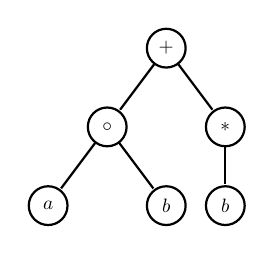
\begin{tikzpicture}[-,shorten >=0.5pt,auto, node distance=1.7cm,
                    thick,every state/.style={thick, minimum size=20pt, scale=0.7}]


  \node[state] at (0,0)         (A)  {$+$};
  \node[state] at (-0.75,-1)    (B)  {$\circ$};
  \node[state] at (0.75,-1)     (C)  {$\ast$};
  \node[state] at (-1.5,-2)     (D)  {$a$};
  \node[state] at (0,-2)        (E)  {$b$};
  \node[state] at (0.75,-2)     (F)  {$b$};
  
  \path (A) edge (B)
            edge (C)
        (B) edge (D)
            edge (E)
        (C) edge (F);

\end{tikzpicture}

\end{minipage}%
\begin{minipage}{.3\textwidth}
  \centering
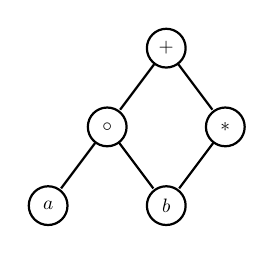
\begin{tikzpicture}[-,shorten >=0.5pt,auto, node distance=1.7cm,
                    thick,every state/.style={thick, minimum size=20pt, scale=0.7}]


  \node[state] at (0,0)         (A)  {$+$};
  \node[state] at (-0.75,-1)    (B)  {$\circ$};
  \node[state] at (0.75,-1)     (C)  {$\ast$};
  \node[state] at (-1.5,-2)     (D)  {$a$};
  \node[state] at (0,-2)        (E)  {$b$};

  
  \path (A) edge (B)
            edge (C)
        (B) edge (D)
            edge (E)
        (C) edge (E);

\end{tikzpicture}

\end{minipage}
\begin{minipage}{.3\textwidth}
  \centering
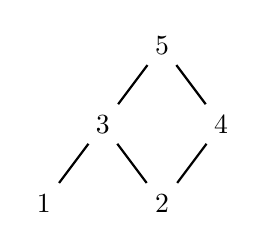
\begin{tikzpicture}[-,shorten >=0.5pt,auto, node distance=1.7cm,
                    thick,every state/.style={thick, minimum size=20pt, scale=0.7}]


  \node at (0,0)         (A)  {$5$};
  \node at (-0.75,-1)    (B)  {$3$};
  \node at (0.75,-1)     (C)  {$4$};
  \node at (-1.5,-2)     (D)  {$1$};
  \node at (0,-2)        (E)  {$2$};

  
  \path (A) edge (B)
            edge (C)
        (B) edge (D)
            edge (E)
        (C) edge (E);

\end{tikzpicture}

\end{minipage}

\end{figure}

\noindent
The semantics of regular expression is generally defined in terms of the language they define:
$$\sema{a}=\{a\};\ \sema{r_1+r_2}=\sema{r_1}\cup\sema{r_2};\ \sema{r_1\circ r_2}=\sema{r_1}\circ \sema{r_2};\ \sema{r^*}=\sema{r}^*$$





Let $w[i,j)$ refer to the subword of $w$ starting from position $i$ and ending at position $j-1$. Also, $w[i,i)=\epsilon$ in this definition. Assume, here that the indexing of word starts from position $0$. 

\begin{definition}{\label{def:match-rel}}

Matching relation $\vdash\subseteq\Sigma^\ast\times \mathcal{R}_\Sigma $ is defined inductively on the structure of a regular expression $r$ in the following manner:
\begin{align*}
&w[i,j)\vdash \epsilon \iff i=j\\
&w[i,j)\vdash a\  \text{where}\ a\in \Sigma \iff w[i,j)=a\\
&w[i,j)\vdash r_1+r_2\ \iff\ w[i,j)\vdash r_1\ \text{or}\ w[i,j)\vdash r_2\\
&w[i,j)\vdash r_1\circ r_2  \iff \exists k\in\mathbb{N}\text{ such that } i\leq k\leq j\text{ and } w[i,k)\vdash r_1 \text{ and } w[k+1,j)\vdash r_2 \\
&w[i,j)\vdash r^* \iff  
\begin{cases}
i=j\text{ or}\\
\exists k\in\mathbb{N} \text{ such that } i< k\leq j \text{ and }w[i,k)\vdash r \text{ and } w[k,j)\vdash r^*
\end{cases}
\end{align*}
\end{definition}

The matching relation $\vdash$ holds true when a word belongs to the language defined by the regular expression. More precisely, we have that ${w[i,j)\vdash r\iff w[i,j)\in\sema{r}}$. This statement can be proved using a simple induction on the structure of $r$. 

Motivated by definition of matching relation, it is possible to design algorithm for checking whether a given word $w$ matches a regular expression $r$, using a \emph{dynamic programming technique}. Let $T_{w}$ be a three dimensional table with $\abs{w}+1$ number of rows and columns both indexed using $0\cdots n$ and the third index is used to denote the subexpression of the expression $r$ for which we are computing the matching relation. The entries of the table have the following meaning.

$$T_w(i,j,r)=1\ \iff w[i,j)\vdash r $$


Given, a regular expression $r$, the table $T_{w}$ is constructed in a iterative manner starting from the portion of the table which refers to the leaf elements of the syntax DAG. These table entries are used for propagating the results to table entries for the internal nodes.\\
\noindent

\begin{itemize}[label=-]
\item For the regular expression $\varepsilon$:\hspace{2pt} $T_{w}(i,j,\varepsilon)=1 \iff i=j$

\item For a leaf node say $a$,\hspace{2pt} $T_{w}(i,j,a)=1 \iff w[i,j)=a$

\item For $+$(union) node, with children $r_1$ and $r_2$:\\$T_w(i,j,r_1+r_2)=1 \text{ if } T_{w}(i,j,r_1)=1 \text{ or } T_w(i,j,r_2)=1$

\item For $\circ$(concat) node, with children $r_1$ and $r_2$:\\$T_w(i,j,r_1\circ r_2)=1 \text{ if } \exists k, i \text{ such that }T_w(i,k,r_1)=1 \text{ and } T_w(k,j,r_2)=1$

\item For $*$(kleene star) node, with a child $r$:\\$T_w(i,j,r^*)=1 \text{ if } \exists k \text{ such that }T_w(i,k,r)=1 \text{ and } T_w(k,j,r^*)=1$
In this case, $T_w$ is filled starting from $(n,n)$th entry up along the columns. 
\end{itemize}
\subsection{The learning problem}
We assume that the data to learn from is given as a pair $\mathcal S = (\mathcal P, \mathcal N)$ consisting of two finite, disjoint sets $\mathcal P, \mathcal N) \subset \Sigma^\ast$ of finite words such that $\mathcal P \cup \mathcal N) \neq \emptyset$.
We call this pair a \emph{sample}.
Moreover, we say that a regular expression $r$ over $\Sigma$ is \emph{consistent} with a sample $\mathcal S = (\mathcal P,\mathcal N)$ if
\begin{enumerate}
	\item $r \vdash u$ for each $u \in \mathcal P$; and
	\item $r \nvdash u$ for each $u \in \mathcal N$.
\end{enumerate}

A possible solution could be to use SAT-solvers to find the regular expression consistent with the given sample. The SAT formula $\varphi_n$ that we feed into the solver has the following structure:

$$\varphi=\varphi^{\text{structure}}_n \wedge  \varphi^{\text{consistency}}_n$$ 
Here, satisfying assignment of $\varphi^{\text{structure}}_n$ provides encoding of a syntax DAG which describes expression of size $n$, while the $\varphi^{\text{consistency}}_n$ checks whether the guessed expression is consistent with the given sample. $\varphi^{\text{structure}}_n$ uses the following variables:

\begin{itemize}[label=$-$]
\item$x_{p,\lambda}$ where $p\in \{1,\cdots, n\}$ and $\lambda\in\Lambda$
\item$l_{p,q}$ where $p\in \{2,\cdots,n\}$ and $q\in\{1,...,p−1\}$
\item$r_{p,q}$ where $p\in \{2,\cdots,n\}$ and $q\in\{1,...,p−1\}$
\end{itemize}
Now, this is how the formula looks like. It is formed by taking conjunction of the following subformulas.

\begin{align}
    [\bigwedge\limits_{1\leq p\leq n} \bigvee\limits_{\lambda \in \Lambda}x_{p,\lambda}]&\wedge[\bigwedge\limits_{1\leq p\leq n}\bigwedge\limits_{\lambda\neq\lambda^{\prime}\in\Lambda}\neg x_{p,\lambda}\vee \neg x_{p,\lambda^{\prime}}]\label{eq:sat1}\\
    [\bigwedge\limits_{2\leq p\leq n} \bigvee\limits_{1\leq q\leq p}l_{p,q}]&\wedge[\bigwedge\limits_{2\leq p\leq n}\bigwedge\limits_{1\leq q\leq q^{\prime}\leq n}\neg l_{p,q}\vee \neg l_{p,q^{\prime}}]\label{eq:sat2}\\
        [\bigwedge\limits_{2\leq p\leq n} \bigvee\limits_{1\leq q\leq p}r_{p,q}]&\wedge[\bigwedge\limits_{2\leq p\leq n}\bigwedge\limits_{1\leq q\leq q^{\prime}\leq n}\neg r_{p,q}\vee \neg r_{p,q^{\prime}}]\label{eq:sat3}\\
    x_{1,\epsilon}&\vee \bigvee\limits_{a\in\Sigma} x_{1, a}\label{eq:sat4}
\end{align}
Subformula~\eqref{eq:sat1} says that each node would be uniquely labelled by an element from $\Lambda$. Subformulas~\eqref{eq:sat2} and~\eqref{eq:sat3} say that each node would have a unique left and right child respectively. Last but not the least, Subformula~\eqref{eq:sat4} says that the first node can have only $\epsilon$ or an alphabet.

First let us consider, for each word $w$ in the given sample, a three dimensional table whose entries are basically variables $y^w_{i,j,p}$, where the indices $i$ and $j$ refers to the substring of the word $w$ and $p$ refers to the sub-expression we are looking at. For simplicity, we assume $m=\abs{w}$. Now, $\varphi^w_n$ is a conjunction of the following subformulas:

\begin{align}
\bigwedge\limits_{1\leq p \leq n}x_{p,\varepsilon}&\rightarrow\Big[\bigwedge\limits_{0\leq i\leq j\leq m }y^w_{i,j,p}\leftrightarrow [i=j]\Big]\label{eq:sat5}\\
\bigwedge\limits_{1\leq p \leq n}\bigwedge\limits_{a\in \Sigma}x_{p,a}&\rightarrow\Big[\bigwedge\limits_{0\leq i\leq j\leq m }
\begin{cases}
y^w_{i,j,p}\text{ if }w[i,j)=a\\
\neg y^w_{i,j,p}\text{ if }w[i,j)\neq a
\end{cases}\Big]\label{eq:sat6}\\
\bigwedge\limits_{\substack{1\leq p \leq n \\ 1\leq q, q^{\prime}\leq p}}x_{p,+}\wedge l_{p,q}\wedge r_{p,q^{\prime}}&\rightarrow\Big[\bigwedge\limits_{\substack{0\leq i \leq j \leq m}}\Big[y^w_{i,j,p}\leftrightarrow y^w_{i,j,q}\vee y^w_{i,j,q^{\prime}}\Big]\Big]\label{eq:sat7}\\  
\bigwedge\limits_{\substack{1\leq p \leq n \\ 1\leq q, q^{\prime}\leq p}}x_{p,\circ}\wedge l_{p,q}\wedge r_{p,q^{\prime}}&\rightarrow\Big[\bigwedge\limits_{\substack{0\leq i\leq j \leq m }}\Big[y^w_{i,j,p}\leftrightarrow \bigvee\limits_{i\leq k\leq j}y^w_{i,k,q}\wedge y^w_{k,j,q^{\prime}}\Big]\Big]\label{eq:sat8} \\
\bigwedge\limits_{\substack{1\leq p \leq n \\ 1\leq q, q^{\prime}\leq p}}x_{p,*}\wedge l_{p,q}&\rightarrow\Big[\bigwedge\limits_{\substack{0\leq i \leq j \leq m}}\Big[y^w_{i,j,p}\leftrightarrow [i=j]\vee \bigvee\limits_{i< k\leq j}y^w_{i,k,q}\wedge y^w_{k,j,p}\Big]\Big] \label{eq:sat9}
\end{align}

The idea for each of these subformulas is motivated by the procedure for filling out the table $T_w$, which in turn essentially uses the way the matching relation has been defined. Using the formula $\varphi^w_n$ for various $w$, we construct $\varphi^\text{consistency}_n$ in the following manner.

\begin{align}
\varphi^\text{consistency}_n=\Big[\bigwedge\limits_{w\in \mathcal P} \varphi_n^{w} \wedge y^w_{0,m,n} \Big]\wedge \Big[\bigwedge\limits_{w\in \mathcal N} \varphi_n^{w} \wedge \neg y^w_{0,m,n} \Big]
\end{align}


Given that we have devised SAT formula for this problem, we utilise it to come up with a simple algorithm using SAT-solvers to find out the smallest regular expression consistent with the sample.
\begin{algorithm}
	\KwIn{A sample $\mathcal S$}
	\DontPrintSemicolon

	\BlankLine
	$n \gets 0$\;
	\Repeat {$\varphi_n^\mathcal S$ is satisfiable, say with model $v$}
	{
		$n \gets n+1$\;
		Construct and solve the formula $\varphi_n^\mathcal S$ using a SAT solver
	}
	\BlankLine
	\Return the regular expression $R^v$\;

	\caption{SAT-based learning algorithm for regular expressions} \label{alg:sat-learner}
\end{algorithm}

\subsection{Proof of correctness}
\begin{claim}
Let $\mathcal{S} = (\mathcal{P}, \mathcal{N})$ be a sample, $n \in \mathbb N \setminus \{ 0 \}$, and $\varphi_n^\mathcal S$ be the propositional formula defined above.
Then, the following holds:
\begin{enumerate}
	\item If there exists a regular expression of size $n$, $R^{\mathcal S}$ that is consistent with $\mathcal S$, then the propositional formula $\varphi_n^\mathcal S$ is satisfiable.
	\item If $v \models \varphi_n^\mathcal S$, then $R^{v}$ is a regular expression of size $n$ that is consistent with $\mathcal S$.
\end{enumerate}
\end{claim}
\begin{proof}
    Using the syntax DAG of the expression $R^{\mathcal S}$ which is indexed using $1\cdots n$, we formulate a valuation $v$ for the propositional variables in $\varphi^{\mathcal S}_n$. We use $R_p^{\mathcal S}$ to refer to the regular expression rooted at the $p^{th}$ node.  
    \begin{itemize}[label=$-$]
    \item We set $v(x_{p,\lambda})=1$ iff the $p^{th}$ node is labelled by $\lambda$.   
    \item We set $v(l_{p,q})=1$ iff $q^{th}$ node is the left child of the $p^{th}$ node and similarly,  $v(r_{p,q})=1$  iff $q^{th}$ node is the right child of the $p^{th}$ node.
    \item We set $v(y^w_{i,j,p})=1$ iff $w[i,j)\vdash R_p^{\mathcal S}$ 
    \end{itemize}
Firstly, it is easy to see that $v\models \varphi_n^{\text{structure}}$, since the formulated valuation ensures the uniqueness of the labels of the nodes as well as that of the left and right children. Moreover, $v\models \varphi^w_n$ for $w\in \mathcal{P}\cup \mathcal{N}$, since, the values of the variables
$y^w_{i,j,p}$ correspond exactly to the valuation of each subexpression $R_i^{\mathcal S}$ on the subword $w[i,j)$. Finally, the fact that $R^{\mathcal S}$ is consistent with $\mathcal S$ implies $v\models y^w_{i,j,p}$ for each $w\in \mathcal P$ and $v\models\neg y^{w}_{i,j,p}$ for each $w\in \mathcal N$. Thus, $v\models \varphi^{\mathcal S}_n$, which proves that $\varphi^{\mathcal S}_n$ is satisfiable.
\\

For the second statement, since, $v\models \varphi^S_n$, we have $v\models \varphi^{\text{structure}}_n$ as well. Hence, the valuation of the variables $x_{p,\lambda}$, $l_{p,q}$, and $r_{p,q}$ encode a syntax DAG from which we obtain the regular expression $R^v$. Again here, we consider $R_p^v$ to be the subexpression of $R^v$ rooted at the $p^{th}$ node. Now, it needs to be shown that $R^v$ is indeed consistent with the sample $\mathcal S$. For that we show, ${v(y^w_{i,j,p})=1 \iff w[i,j)\vdash R^v_p}$ for any $i$,$j\in \{0,\cdots, m\}$ where $m=\abs{w}+1$ and $p\in \{0,\cdots, n\}$. This can be done using induction on the structure of $R^v$.

\begin{itemize}[label=$-$]
    \item \textit{Base case $R^v_p=\varepsilon$}: In this case, $v(x_{p,\epsilon})=1$, which leads to the following implications:
    \begin{align*}
    v(y^w_{i,j,p})=1&\iff i=j  &&\text{[Using Subformula~\eqref{eq:sat5}]}\\
                    &\iff w[i,j)\vdash\varepsilon &&\text{[Using Def.~\ref{def:match-rel}]}
    \end{align*}
    \item \textit{Base case $R^v_p=a$}: In this case, $v(x_{p,a})=1$ and this leads to the following implications: 
    \begin{align*}
    v(y^w_{i,j,p})=1 &\iff w[i,j)=a &&\text{[Using Subformula~\eqref{eq:sat6}]}\\
                     &\iff w[i,j)\vdash a&&\text{[Using Def.~\ref{def:match-rel}]}
    \end{align*}
    \item \textit{Case $R^v_p=R^v_q+R^v_{q^{\prime}}$}: In this case, $v(x_{p,+})$, $v(l_{p,q})$, $v(r_{p,q^{\prime}})$ are all set to 1, and this leads to the following implications:
    \begin{align*}
    v(y^w_{i,j,p})=1 &\iff v(y^w_{i,j,q})=1 \text{ or } v(y^w_{i,j,q^{\prime}})=1 &&\text{[Using Subformula~\eqref{eq:sat7}]}\\
    &\iff w[i,j)\vdash R^v_q\text{ or } w[i,j)\vdash R^v_{q^{\prime}}&&\text{[Using ind. hypothesis]}\\
    &\iff w[i,j)\vdash R^v_q+R^v_{q^{\prime}}&&\text{[Using Def.~\ref{def:match-rel}]}
    \end{align*}
    \item \textit{Case $R^v_p=R^v_q\circ R^v_{q^{\prime}}$}: In this case, $v(x_{p,\circ})$, $v(l_{p,q})$, $v(r_{p,q^{\prime}})$ are all set to 1 and this leads to the following implications:
    \begin{align*}
    v(y^w_{i,j,p})=1 &\iff \exists k\in \mathbb{N},\ 1\leq k\leq m, v(y^w_{i,k,q})=1 \text{ and } v(y^w_{k,j,q^{\prime}})=1 &&\text{[Using Subformula~\eqref{eq:sat8}]}\\
    &\iff \exists k\in \mathbb{N},\ 1\leq k\leq m, w[i,k)\vdash R^v_q \text{ and } w[k,j)\vdash R^v_{q^{\prime}}&&\text{[Using ind. hypothesis]}\\
    &\iff w[i,j)\vdash R^v_q\circ R^v_{q^{\prime}}&&\text{[Using Def.~\ref{def:match-rel}]}
    \end{align*}
    \item \textit{Case $R^v_p=(R^v_q)^{*}$}: In this case, $v(x_{p,*})$ and $v(l_{p,q})$ are set to 1 and this leads to the following implications:
     \begin{align*}
    v(y^w_{i,j,p})=1 &\iff 
    \begin{cases} 
    i=j \text{ or}\\ 
    \exists k\in \mathbb N,\ 1\leq k\leq m,\ v(y^w_{i,k,q})=1 \text{ and }v(y^w_{k,j,p})=1
    \end{cases} &&\text{[Using Subformula~\eqref{eq:sat9}]}\\
    &\iff     
    \begin{cases} 
    i=j \text{ or}\\ 
    \exists k\in \mathbb N,\ 1\leq k\leq m,\ w[i,k)\vdash R^v_q \text{ and }w[k,j)\vdash (R^v_{q})^*
    \end{cases}&&\text{[Using ind. hypothesis]}\\
    &\iff w[i,j)\vdash (R^v_q)^*&&\text{[Using Def.~\ref{def:match-rel}]}
    \end{align*}
    
    Here, we assumed that $v(y^w_{k,j,p})=1$ iff $w[k,j)\vdash R^v_{p}$ in the second step, which cannot be deduced from the induction on the structure of $R^v_p$. This we obtained using another level of induction, which is on the length of the subword that matches $R^v_{p}$. More precisely, we induct on $k$ which ranges from $j$ to $i+1$, where by induction hypothesis, it is assumed that 
    $$v(y^w_{k,j,p})=1 \iff w[k,j)\vdash R^v_{p}\quad \forall k,\ i<k\leq j$$
    The base case occurs when $k=j$, and then, we have 
    ${v(y^w_{k,j,p})=1 \iff k=j  \iff w[k,j)\vdash R^v_{p}}$.

    
\end{itemize}

\end{proof}
\chapter{Learning $\omega-$Regular Expressions}


In this chapter, we present SAT-based learning algorithm for learning $\omega-$Regular expressions from a sample of positive and negative infinite words. 

\section{$\omega$-Regular expression}
An $\omega$-regular expression $r_\omega$ is an expression with the following grammar:
\begin{equation*}
    r_\omega:=r^\omega \mid r\circ_\omega r_\omega \mid r_\omega+_\omega r_\omega
\end{equation*}
where, $r$ is a regular expression as described in Section~\ref{subsec:regex-def}. Let the set of $\omega-$regular expressions be denoted by $\mathcal{R}_{\Sigma}^{\omega}$.
Again here, a $\omega-$regular expression can be represented in the form of a syntax tree or a syntax DAG, similar to ones for regular expressions. The only difference here is that the nodes of the syntax tree and the syntax DAG are labelled by elements from $\Lambda_\omega=\Lambda\cup\{\omega, +_\omega, \circ_\omega\}$.  The semantics of a $\omega-$regular expression is as usual defined as the language they defined, which is obtained in the following manner:
\begin{equation*}
    \sema{r^\omega}=\sema{r}^\omega;\ \sema{r\circ_\omega r_\omega}=\sema{r}\circ_\omega\sema{r_{\omega}};\ \sema{r_\omega+_{\omega}r_\omega^{\prime}}=\sema{r_\omega}\cup \sema{r_\omega^{\prime}}
\end{equation*}
It should be noted that $r^\omega$ is well defined only when $\epsilon\notin \sema{r}$, since otherwise, $\sema{r^\omega}$ might contain invalid infinite words.
Now, let us look at some results regarding membership of ultimately periodic words in languages defined by $\omega-$regular expressions. In the following results, we assume $u$ and $v$ are words in $\Sigma^*$ and $r$ is a regular expression in $\mathcal{R}_\Sigma$, such that $\epsilon\notin \sema{r}$. Moreover, assume that the minimal DFA of $\sema{r}$ has size $n$.

\begin{prop}{\label{prop:w-membership}}
$uv^{\omega}\in \sema{r^{\omega}}\iff \exists i, j\in \mathbb{N},\ \abs{u}<i<j,\ uv^\omega[0,i)\in \sema{r^+}  \text{ and } uv^\omega[i,j) \in \sema{r^+} \text{ where } j\equiv i\mod \abs{v}$.
\end{prop}
\begin{proof}
 ($\Rightarrow$) From the semantics of $\omega$-regular expressions, we have $uv^\omega\in \sema{r^\omega}\implies uv^\omega\in\sema{r}^\omega$. Hence, there exists an infinite sequence of natural numbers $i_1, i_2, i_3, \ldots$ satisfying ${\abs{u}<i_1<i_2<\ldots}$ such that $uv^\omega[0,i_1)\in \sema{r^+}$ and from then on $uv^\omega[i_1,i_2)\in \sema{r}$, $uv^\omega[i_2,i_3)\in \sema{r}$ and so on. Since, $i_0,i_1,i_2, \ldots$ is an infinite sequence, it is possible to find numbers $i$ and $j$ in the sequence, such that $j\equiv i \mod \abs{v}$ using pigeonhole principle. Now, clearly, $uv^\omega[0,i)\in \sema{r^+}$ and $uv^\omega[i,j)\in \sema{r^+}$, since $i$ and $j$ belong to the sequence.

($\Leftarrow$) Let $uv^\omega[0,i)=v_1$ and $uv^\omega[i,j)=v_2$, where both $uv^\omega[0,i)$ and $uv^\omega[i,j)$ satisfy the properties mentioned in the lemma. It is an easy observation that $v_1v_2^{\omega}=uv^\omega$. As we already know ${v_1\in \sema{r^+}}$ and $v_2\in \sema{r^+}$, we can conclude that ${v_1v_2^\omega \in \sema{r^+}\circ \sema{r^+}^\omega \implies v_1v_2^\omega
\in\sema{r^\omega}\implies uv^\omega \in \sema{r^\omega}}$. 
\end{proof}
\begin{lemma}\label{lem:bound-r}
$v^{\omega}\in \sema{r^\omega}\iff\exists i \in \mathbb{N},\ v^\omega[0,i)\in \sema{r^{\abs{v}+1}}$.
\end{lemma}

\begin{proof}
$(\Rightarrow)$  Since, $v^\omega\in \sema{r}^\omega$, for any natural number $n$, there is a prefix $v^\omega[0,i)$ of $v^\omega$ such that $v^\omega[0,i)\in \sema{r^n}$. Therefore, it holds true for $n=\abs{v}+1$ as well.

($\Leftarrow$) Here, we have $v^\omega[0,i)\in \sema{r^{\abs{v}+1}}$ for some $i\in \mathbb{N}$. Therefore, we can find a finite sequence of distinct natural numbers $i_1, i_2, \ldots, i_{\abs{v}+1}$, where $i_{\abs{v}+1}=i$ and also, $v^\omega[0,i_1)\in \sema{r}$, $v^\omega[i_1,i_2)\in \sema{r}$ and so on. Now, notice that it is possible to find numbers $i^{\prime}$, $j^{\prime}$ with $i^\prime<j^\prime$, in the sequence such that $j^{\prime}\equiv i^{\prime} \mod \abs{v}$ using pigeonhole principle(Since, the sequence contains more than $\abs{v}$ elements). Consequently, we have $v^\omega[0,i^{\prime})\in\sema{r^+}$, $v^\omega[i^{\prime},j^{\prime})\in\sema{r^+}$ and $j^{\prime}\equiv i^{\prime} \mod \abs{v}$, which gives us $v^\omega\in\sema{r^\omega}$ straightaway using Prop.~\ref{prop:w-membership}.
\end{proof}
\begin{corollary}\label{cor:bound-r-uv}
Let $uv^{\omega}\in \sema{r^\omega}$ such that for some $i> \abs{u}$, $uv^\omega[0,i)\in\sema{r}$ and $uv^\omega[i,\infty)\in\sema{r^\omega}$. Then, $\exists j \in \mathbb{N},\ j>i,$ such that $uv^\omega[0,j)\in \sema{r^{\abs{v}+1}}$
\end{corollary}
The proof for this proceeds exactly the same way as Lemma~\ref{lem:bound-r}. The next lemma shows how the length of each match can be bounded.
\begin{figure}
    \centering
\tikzset{every picture/.style={line width=0.75pt}} %set default line width to 0.75pt        

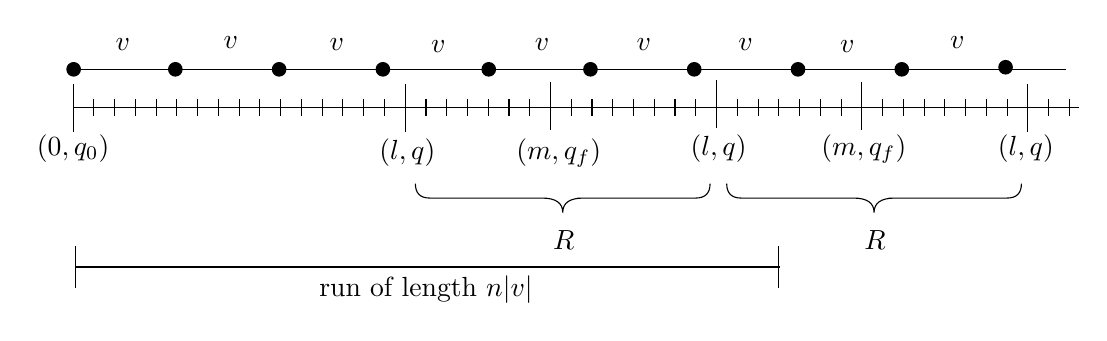
\begin{tikzpicture}[x=0.75pt,y=0.75pt,yscale=-1,xscale=1]
%uncomment if require: \path (0,300); %set diagram left start at 0, and has height of 300

%Straight Lines [id:da9738540502468893] 
\draw    (101,125) -- (585.5,125) (111,121) -- (111,129)(121,121) -- (121,129)(131,121) -- (131,129)(141,121) -- (141,129)(151,121) -- (151,129)(161,121) -- (161,129)(171,121) -- (171,129)(181,121) -- (181,129)(191,121) -- (191,129)(201,121) -- (201,129)(211,121) -- (211,129)(221,121) -- (221,129)(231,121) -- (231,129)(241,121) -- (241,129)(251,121) -- (251,129)(261,121) -- (261,129)(271,121) -- (271,129)(281,121) -- (281,129)(291,121) -- (291,129)(301,121) -- (301,129)(311,121) -- (311,129)(321,121) -- (321,129)(331,121) -- (331,129)(341,121) -- (341,129)(351,121) -- (351,129)(361,121) -- (361,129)(371,121) -- (371,129)(381,121) -- (381,129)(391,121) -- (391,129)(401,121) -- (401,129)(411,121) -- (411,129)(421,121) -- (421,129)(431,121) -- (431,129)(441,121) -- (441,129)(451,121) -- (451,129)(461,121) -- (461,129)(471,121) -- (471,129)(481,121) -- (481,129)(491,121) -- (491,129)(501,121) -- (501,129)(511,121) -- (511,129)(521,121) -- (521,129)(531,121) -- (531,129)(541,121) -- (541,129)(551,121) -- (551,129)(561,121) -- (561,129)(571,121) -- (571,129)(581,121) -- (581,129) ;


%Straight Lines [id:da13702797169170655] 
\draw    (101,114) -- (101,137) ;


%Straight Lines [id:da8041648978491207] 
\draw    (261,114) -- (261,137) ;


%Straight Lines [id:da6595616096690307] 
\draw    (411,112) -- (411,135) ;


%Straight Lines [id:da3060502963477655] 
\draw    (331,113) -- (331,136) ;


%Shape: Brace [id:dp2255019364812435] 
\draw   (265.89,161.78) .. controls (265.89,166.45) and (268.22,168.78) .. (272.89,168.78) -- (326.89,168.78) .. controls (333.56,168.78) and (336.89,171.11) .. (336.89,175.78) .. controls (336.89,171.11) and (340.22,168.78) .. (346.89,168.78)(343.89,168.78) -- (400.89,168.78) .. controls (405.56,168.78) and (407.89,166.45) .. (407.89,161.78) ;

%Straight Lines [id:da2372877431070176] 
\draw    (561,114) -- (561,137) ;


%Straight Lines [id:da10606170516071167] 
\draw    (481,113) -- (481,136) ;


%Straight Lines [id:da6169757431905829] 
\draw    (441,192) -- (441,212) ;


%Straight Lines [id:da5979976123216078] 
\draw    (102.5,202) -- (441.5,202) ;



%Straight Lines [id:da6446637744519785] 
\draw    (102,192) -- (102,212) ;


%Shape: Brace [id:dp7367618017805307] 
\draw   (415.89,161.78) .. controls (415.89,166.45) and (418.22,168.78) .. (422.89,168.78) -- (476.89,168.78) .. controls (483.56,168.78) and (486.89,171.11) .. (486.89,175.78) .. controls (486.89,171.11) and (490.22,168.78) .. (496.89,168.78)(493.89,168.78) -- (550.89,168.78) .. controls (555.56,168.78) and (557.89,166.45) .. (557.89,161.78) ;

%Straight Lines [id:da5097494136295723] 
\draw    (100.5,106.75) -- (579.5,106.75) ;


%Shape: Circle [id:dp7181991198411304] 
\draw  [color={rgb, 255:red, 0; green, 0; blue, 0 }  ,draw opacity=1 ][fill={rgb, 255:red, 0; green, 0; blue, 0 }  ,fill opacity=1 ] (98,106.75) .. controls (98,104.96) and (99.46,103.5) .. (101.25,103.5) .. controls (103.04,103.5) and (104.5,104.96) .. (104.5,106.75) .. controls (104.5,108.54) and (103.04,110) .. (101.25,110) .. controls (99.46,110) and (98,108.54) .. (98,106.75) -- cycle ;
%Shape: Circle [id:dp019890023544648194] 
\draw  [color={rgb, 255:red, 0; green, 0; blue, 0 }  ,draw opacity=1 ][fill={rgb, 255:red, 0; green, 0; blue, 0 }  ,fill opacity=1 ] (147,106.75) .. controls (147,104.96) and (148.46,103.5) .. (150.25,103.5) .. controls (152.04,103.5) and (153.5,104.96) .. (153.5,106.75) .. controls (153.5,108.54) and (152.04,110) .. (150.25,110) .. controls (148.46,110) and (147,108.54) .. (147,106.75) -- cycle ;
%Shape: Circle [id:dp8843951700933347] 
\draw  [color={rgb, 255:red, 0; green, 0; blue, 0 }  ,draw opacity=1 ][fill={rgb, 255:red, 0; green, 0; blue, 0 }  ,fill opacity=1 ] (197,106.75) .. controls (197,104.96) and (198.46,103.5) .. (200.25,103.5) .. controls (202.04,103.5) and (203.5,104.96) .. (203.5,106.75) .. controls (203.5,108.54) and (202.04,110) .. (200.25,110) .. controls (198.46,110) and (197,108.54) .. (197,106.75) -- cycle ;
%Shape: Circle [id:dp03492152069054] 
\draw  [color={rgb, 255:red, 0; green, 0; blue, 0 }  ,draw opacity=1 ][fill={rgb, 255:red, 0; green, 0; blue, 0 }  ,fill opacity=1 ] (247,106.75) .. controls (247,104.96) and (248.46,103.5) .. (250.25,103.5) .. controls (252.04,103.5) and (253.5,104.96) .. (253.5,106.75) .. controls (253.5,108.54) and (252.04,110) .. (250.25,110) .. controls (248.46,110) and (247,108.54) .. (247,106.75) -- cycle ;
%Shape: Circle [id:dp5175514544423168] 
\draw  [color={rgb, 255:red, 0; green, 0; blue, 0 }  ,draw opacity=1 ][fill={rgb, 255:red, 0; green, 0; blue, 0 }  ,fill opacity=1 ] (298,106.75) .. controls (298,104.96) and (299.46,103.5) .. (301.25,103.5) .. controls (303.04,103.5) and (304.5,104.96) .. (304.5,106.75) .. controls (304.5,108.54) and (303.04,110) .. (301.25,110) .. controls (299.46,110) and (298,108.54) .. (298,106.75) -- cycle ;
%Shape: Circle [id:dp4499225794259555] 
\draw  [color={rgb, 255:red, 0; green, 0; blue, 0 }  ,draw opacity=1 ][fill={rgb, 255:red, 0; green, 0; blue, 0 }  ,fill opacity=1 ] (347,106.75) .. controls (347,104.96) and (348.46,103.5) .. (350.25,103.5) .. controls (352.04,103.5) and (353.5,104.96) .. (353.5,106.75) .. controls (353.5,108.54) and (352.04,110) .. (350.25,110) .. controls (348.46,110) and (347,108.54) .. (347,106.75) -- cycle ;
%Shape: Circle [id:dp6528014662581125] 
\draw  [color={rgb, 255:red, 0; green, 0; blue, 0 }  ,draw opacity=1 ][fill={rgb, 255:red, 0; green, 0; blue, 0 }  ,fill opacity=1 ] (397,106.75) .. controls (397,104.96) and (398.46,103.5) .. (400.25,103.5) .. controls (402.04,103.5) and (403.5,104.96) .. (403.5,106.75) .. controls (403.5,108.54) and (402.04,110) .. (400.25,110) .. controls (398.46,110) and (397,108.54) .. (397,106.75) -- cycle ;
%Shape: Circle [id:dp7506574991528185] 
\draw  [color={rgb, 255:red, 0; green, 0; blue, 0 }  ,draw opacity=1 ][fill={rgb, 255:red, 0; green, 0; blue, 0 }  ,fill opacity=1 ] (447,106.75) .. controls (447,104.96) and (448.46,103.5) .. (450.25,103.5) .. controls (452.04,103.5) and (453.5,104.96) .. (453.5,106.75) .. controls (453.5,108.54) and (452.04,110) .. (450.25,110) .. controls (448.46,110) and (447,108.54) .. (447,106.75) -- cycle ;
%Shape: Circle [id:dp360058250991258] 
\draw  [color={rgb, 255:red, 0; green, 0; blue, 0 }  ,draw opacity=1 ][fill={rgb, 255:red, 0; green, 0; blue, 0 }  ,fill opacity=1 ] (497,106.75) .. controls (497,104.96) and (498.46,103.5) .. (500.25,103.5) .. controls (502.04,103.5) and (503.5,104.96) .. (503.5,106.75) .. controls (503.5,108.54) and (502.04,110) .. (500.25,110) .. controls (498.46,110) and (497,108.54) .. (497,106.75) -- cycle ;
%Shape: Circle [id:dp3510785942107961] 
\draw  [color={rgb, 255:red, 0; green, 0; blue, 0 }  ,draw opacity=1 ][fill={rgb, 255:red, 0; green, 0; blue, 0 }  ,fill opacity=1 ] (547,105.75) .. controls (547,103.96) and (548.46,102.5) .. (550.25,102.5) .. controls (552.04,102.5) and (553.5,103.96) .. (553.5,105.75) .. controls (553.5,107.54) and (552.04,109) .. (550.25,109) .. controls (548.46,109) and (547,107.54) .. (547,105.75) -- cycle ;

% Text Node
\draw (262,147) node  [align=left] {$\displaystyle ( l,q)$};
% Text Node
\draw (101,145) node  [align=left] {$\displaystyle ( 0,q_{0})$};
% Text Node
\draw (412,145) node  [align=left] {$\displaystyle ( l,q)$};
% Text Node
\draw (335,147) node  [align=left] {$\displaystyle ( m,q_{f})$};
% Text Node
\draw (337.39,188.78) node  [align=left] {$\displaystyle R$};
% Text Node
\draw (560,145) node  [align=left] {$\displaystyle ( l,q)$};
% Text Node
\draw (482,145) node  [align=left] {$\displaystyle ( m,q_{f})$};
% Text Node
\draw (271,213) node  [align=left] {run of length $\displaystyle n\abs{v}$};
% Text Node
\draw (487.39,188.78) node  [align=left] {$\displaystyle R$};
% Text Node
\draw (125,95) node  [align=left] {$\displaystyle v$};
% Text Node
\draw (177,94) node  [align=left] {$\displaystyle v$};
% Text Node
\draw (228,95) node  [align=left] {$\displaystyle v$};
% Text Node
\draw (277,96) node  [align=left] {$\displaystyle v$};
% Text Node
\draw (327,95) node  [align=left] {$\displaystyle v$};
% Text Node
\draw (376,95) node  [align=left] {$\displaystyle v$};
% Text Node
\draw (425,95) node  [align=left] {$\displaystyle v$};
% Text Node
\draw (474,96) node  [align=left] {$\displaystyle v$};
% Text Node
\draw (527,94) node  [align=left] {$\displaystyle v$};


\end{tikzpicture}


    \caption{The run of the DFA of $\sema{r}$ on $v^\omega[i,j)$, where $R$ is the repeating run staring at $(l,q)$. The first occurrence of $R$ happens within $n\abs{v}+1$ steps and hence, the first occurrence of state $q_f$ also happens within that many steps.}
    \label{fig:lemma3}
\end{figure}

\begin{lemma}\label{lem:bound-len_match}
$v^{\omega}[i,j)\in \sema{r}\implies \exists k\in\mathbb{N},\ k-i\leq n\abs{v} \text{ such that } v^\omega[i,k)\in \sema{r} \text{ and } k\equiv j \mod \abs{v}$, where $n$ is the size of the minimal DFA for $\sema{r}$.
\end{lemma}
\begin{proof}
If $j-i\leq n\abs{v}$, we are done, since we simply take $k=j$. On the other hand, if $j-i>n\abs{v}$, finding the suitable $k$ is a bit more involved. Firstly, since, $v^{\omega}[i,j)\in \sema{r}$, there is an accepting run of the DFA $\mathcal{A}$ for $\sema{r}$ on $v^{\omega}[i,j)$, which is of length greater than $n\abs{v}$. Now, we look at this run of $\mathcal{A}$ on $v^\omega[i,j)$. Fig \ref{fig:lemma3} provides a pictorial depiction of the run. Here we consider the run to be a sequence of tuples of the form $(m,q)$, where the first entry refers to the position in $v$ which will be read next and the second entry refers to the state of the automaton at that instant. Hence, it is easy to observe that any run longer than $n\abs{v}$ would mean that there exists a tuple which repeats itself during the run, due to pigeonhole principle. Let $(l,q)$ be the tuple which repeats itself and let the run starting at the first occurrence of $(l,q)$ to the next, be referred to as $R$. Notice that due to the deterministic nature of the automaton, $R$ repeats itself during the rest of the run. Hence, if a final state $q_f$ occurs after $n\abs{v}$ steps, there must be a tuple $(m, q_f)$ which belongs to the run $R$. Clearly, $(m, q_f)$ must have been also visited during the first occurrence of $R$, which happened within $n\abs{v}$ steps. Thus, we get a prefix $v^\omega[i,k)\in \sema{r}$, which has length less than $n\abs{v}$. Moreover, $v^\omega[i,j)$ and $v^\omega[i,k)$ terminate at the same position in $v$, meaning $k\equiv j \mod \abs{v}$.


\end{proof}

\begin{corollary}\label{cor:bound-length_match_uv}
$uv^{\omega}[i,j)\in \sema{r}, \text{ where } i<\abs{u}< j \implies \exists k\in\mathbb{N},\ \abs{u}<k\leq\abs{u}+n\abs{v} \text{ such that } uv^\omega[i,k)\in \sema{r} \text{ and } k\equiv j \mod \abs{v}$.
\end{corollary}

The proof for this statement goes along the same lines as Lemma \ref{lem:bound-len_match}. Finally, having these results, it is possible to verify whether an infinite word(ultimately periodic word in this case) actually belongs to the language of regular expression by checking only a finite portion of the word. This turns out to be useful in constructing table

\begin{theorem}{\label{thm:bounded-w-membership}}
$v^{\omega}\in \sema{r^{\omega}}\iff \exists i, j\in \mathbb{N},\ 0<i<j\leq n\abs{v}+n\abs{v}^2\ v^\omega[0,i)\in \sema{r^+}  \text{ and } v^\omega[i,j) \in \sema{r^+} \text{ where } j\equiv i\mod \abs{v}$
\end{theorem}
\begin{proof}
($\Leftarrow$) This can be seen directly from Prop.~\ref{prop:w-membership}, assuming $u=\epsilon$.

($\Rightarrow$) Using Lemma \ref{lem:bound-r}, there exists some $i^{\prime}$ such that $v^\omega[0,i^{\prime})\in \sema{r^{\abs{v}+1}}$. As a result, we can generate a sequence of distinct natural numbers, $i_1,\ldots, i_{\abs{v}+1}$, with $i_{\abs{v}+1}=i^{\prime}$ such that $v^\omega[0,i_1)\in\sema{r}$, $v^\omega[i_1,i_2)\in \sema{r}$ and so on. Now, we can find another sequence $j_1, \ldots, j_{\abs{v}+1}$ with  $j_{\abs{v}+1}$, which satisfy all the properties that the sequence of $i'$s satisfy and additionally have $j_1\leq n\abs{v}$, $j_2-j_1\leq n\abs{v}$, so on and also, $j_1\equiv i_1 \mod {\abs{v}},$ $j_2\equiv i_2 \mod \abs{v}$, so on. This is a direct consequence of Lemma \ref{lem:bound-len_match}. It is easy to see that $j_{\abs{v}}\leq n\abs{v}+n\abs{v}^2$. Moreover, we can again find some $i$ and $j$ in this sequence such that $j\equiv i \mod \abs{v}$ and clearly, $v^\omega[0,i) \in \sema{r^+}$ and $v^\omega[i,j) \in \sema{r^+}$.
\end{proof}


\begin{theorem}
$uv^\omega\in \sema{r^\omega}\iff \exists i, j\in \mathbb{N},\ \abs{u}<i<j\leq \abs{u}+n\abs{v}+n\abs{v}^2\ uv^\omega[0,i)\in \sema{r^+}  \text{ and } uv^\omega[i,j) \in \sema{r^+} \text{ where } j\equiv i\mod \abs{v}$
\end{theorem}

\begin{proof}
($\Leftarrow$) This can be seen directly from Prop. \ref{prop:w-membership}.

($\Rightarrow$) When $uv^\omega\in \sema{r^\omega}$, there could be two possible cases arising from how $uv^\omega$ matches $r^\omega$.  
\begin{itemize}[label=$-$]
    \item First case would be one in which $u\in\sema{r^+}$ and $v^\omega\in \sema{r^\omega}$. In this case, Theorem \ref{thm:bounded-w-membership} can be applied directly to obtain the result. 
    \item In the second case, $\exists i^\prime, j^\prime \in \mathbb{N}$ with $i^\prime<\abs{u}<j^\prime$, such that, $uv^\omega[0,i^\prime)\in\sema{r^+},\ uv^\omega[i^\prime,j^\prime)\in\sema{r}, \text{ and } uv^\omega[j^\prime,\infty)\in \sema{r^\omega}$. Now, it can be seen that infix $uv^\omega[i^\prime,\infty)$ satisfies the conditions of Corollary~\ref{cor:bound-r-uv}. Hence, there is some $k^\prime>j^\prime$, such that $uv^\omega[i^\prime,k^\prime)\in \sema{r^{\abs{v}+1}}$. As a result, we can generate a sequence of distinct natural numbers $i_1,\ldots, i_{\abs{v}+1}$, with $i_1=j^\prime$ and $i_{\abs{v}+1}=k^\prime$ such that $uv^\omega[i^\prime,i_1)\in\sema{r},uv^\omega[i_1,i_2)\in\sema{r}$ and so on. Combining results of  Corollary~\ref{cor:bound-length_match_uv} and Lemma~\ref{lem:bound-len_match}, we can find another sequence $j_1,j_2\ldots j_{\abs{v}+1}$ which satisfy the properties of the sequence of $i'$s and additionally have $j_1\leq\abs{u}+n\abs{v}$, $j_2-j_1\leq n\abs{v}$, $j_3-j_2\leq n\abs{v}$, so on and also, $j_1=i_1\mod{\abs{v}}$, $j_2=i_2\mod{\abs{v}}$, so on. It is easy to see that $j_{\abs{v}+1}\leq \abs{u}+n\abs{v}+n\abs{v}^2$. Moreover, in this sequence  we can find some $i$ and $j$ such that $j \equiv i \mod{\abs{v}}$ and clearly, $uv^\omega[0,i)\in\sema{r^+}$ and $uv^\omega[i,j)\in\sema{r^+}$.
\end{itemize}

\end{proof}

Motivated by the above results, we define the matching relation for infinite words which would help us to algorithmically check the matching of a ultimately periodic word with a $\omega-$ regular expression.

\begin{definition}
The matching relation $\vdash$ for finite words with regular expressions, could be extended to account for matching of ultimately periodic words with $\omega$-regular expressions as well. Here, $n$ refers to the size of the minimal DFA of $\sema{r}$ in all the cases.

 \begin{align*}
        &v^\omega[i,\infty)\vdash  r^\omega   \iff  \exists j, k\in \mathbb{N},\ i<j<k\leq i+n\abs{v}+n\abs{v}^2,\ v^\omega[i,j)\vdash r^+  \text{ and } v^\omega[j,k) \vdash r^+ \text{ where } k\equiv j\mod \abs{v}\\
    &v^\omega[i,\infty) 
    \vdash r\circ r_\omega \iff  \exists j\in \mathbb{N},\ j\leq n\abs{v},\ v^\omega[i,j)\vdash r \text{ and } v^\omega[j,\infty)\vdash r_\omega\\
    &v^\omega[i,\infty) \vdash r_\omega+ r_\omega^{\prime} \iff   v^\omega[i,\infty)\vdash r_\omega \text{ or } v^\omega[i,\infty)\vdash r_\omega^{\prime}
\end{align*}
 \begin{align*}
        &uv^\omega[i,\infty)\vdash  r^\omega   \iff  \exists j, k\in \mathbb{N},\ i+\abs{u} < j<k\leq i+\abs{u}+n\abs{v}+n\abs{v}^2,\ \\&\hspace{6.5cm} uv^\omega[i,j)\vdash r^+  \text{ and } uv^\omega[j,k) \vdash r^+ \text{ where } k\equiv j\mod \abs{v}\\
    &uv^\omega[i,\infty) \vdash r\circ r_\omega \iff  \exists j\in \mathbb{N},\ i\leq j\leq\abs{u}+ n\abs{v},\ uv^\omega[0,i)\vdash r \text{ and } uv^\omega[i,\infty)\vdash r_\omega\\
    &uv^\omega[i,\infty) \vdash r_\omega+ r_\omega^{\prime} \iff   uv^\omega[i,\infty)\vdash r_\omega \text{ or } uv^\omega[i,\infty)\vdash r_\omega^{\prime}
\end{align*}

\end{definition}
Firstly, it needs to be checked whether the matching relation satisfies ${v^\omega[i,\infty)\vdash r_\omega \iff v^\omega[i,\infty)\in \sema{r_\omega}}$.
The proof goes via induction on the structure of the the $\omega-$regular expression. 
\begin{itemize}[label=$-$]
\item \textit{Case $r_\omega=r^\omega:$} This follows directly from Theorem \ref{thm:bounded-w-membership}
\item \textit{Case $r_\omega=r\circ r^{\prime}_\omega:$} Consider the following implications:
\begin{align*}
    v^\omega[i,\infty) \vdash r\circ r^{\prime}_\omega &\iff \exists j\in \mathbb{N},\ j\leq n\abs{v},\ v^\omega[i,j)\vdash r \text{ and } v^\omega[j,\infty)\vdash r_\omega\\
    &\iff\exists j\in \mathbb{N},\ v^\omega[i,j)\in r \text{ and } v^\omega[j,\infty)\in \sema{r_\omega^{\prime}}&& \text{[Using induction hypothesis]}\\
    &\iff\exists j\in \mathbb{N},\ v^\omega[i,j)\in \sema{r} \text{ and } v^\omega[j,\infty)\in \sema{r_\omega}&& \text{[Using Lemma \ref{lem:bound-len_match}]}\\
    &\iff v^\omega[i,\infty)\in \sema{r_\omega}
\end{align*}
\item Case $r_\omega=r^{\prime}_\omega+r^{\prime\prime}_\omega:$ Consider the following implications:
\begin{align*}
        v^\omega[i,\infty) \vdash r^{\prime}_\omega + r^{\prime\prime}_\omega &\iff v^\omega[i,\infty)\vdash r_\omega \text{ or } v^\omega[i,\infty)\vdash r_\omega^{\prime}  \\
    &\iff v^\omega[i,\infty)\in \sema{r_\omega} \text{ or } v^\omega[i,\infty)\in \sema{r_\omega^{\prime}}\\
    &\iff v^\omega[i,\infty)\in \sema{r_\omega}
\end{align*}
\end{itemize}
Unlike regular expression, the construction of the tables for algorithmically checking matching of a $\omega-$regular expression with a $\omega-$word needs a slightly different approach. There are two types of tables that need to be maintained for each node 
\chapter{Learning Program Specification Language}

\section{PSL Formulas}
 
PSL subsumes LTL and has an increased expressive power: While the expressive power of LTL is that of star-free $\omega$-regular expressions, the expressive power of PSL is the same as the full class of $\omega$-regular expressions. As PSL is a widely used standard it contains a large amount of derived operators; we concentrate here only on a subset of operators that suffice to obtain the expressive power of $\omega$-regular expressions. We call this subset corePSL. The syntax of  corePSL is given by the following grammar: 
$$\varphi ::= p ~|~ \varphi_1 \vee \varphi_2 ~|~ \neg \varphi ~|~ \pslnext \varphi ~|~ \varphi_1 \psluntil \varphi_2 ~|~ r \triggers \varphi$$
where $p\in \AP$, where Let $\AP$ be a set of atomic propositions and  $r$ is a regular expression over $2^\AP$. % that does not accept the empty word.
The operator $\triggers$ is called \emph{suffix implication} or \emph{triggers}.
\paragraph{Abbreviations}
We mention only the main abbreviations related to the suffix implication operator.
\[
\begin{array}{rcl}
r \xtriggers \varphi &::= & r \triggers (true \cdot \varphi) \\ 
r \followedby \varphi &::= & \neg (r \triggers \neg \varphi) \\
%r \xfollowedby \varphi ::= & \neg (r \xtriggers \neg \varphi) \\
r &::= & r \followedby \mathit{true}
\end{array}
\]

\subsubsection{Semantics}
Given a word $w \in (2^{\AP})^\omega$ and a corePSL formula $\varphi$, we define the relation $w \modelspsl \varphi$ (read ``$w$ satisfies $\varphi$'') similarly to the way it is defined for LTL. 
\begin{align*}
&w \modelspsl p \text{ if }p \in w(0)\\
&w \modelspsl \neg \varphi \text{ iff } w \modelspsl \varphi\\
&w\modelspsl \varphi \vee \psi \text{ iff } w \modelspsl \varphi \text{ or } w \modelspsl \varphi\\
&w \modelspsl \pslnext \varphi \text{ iff } w[1,\infty] \modelspsl \varphi\\
&w \modelspsl \varphi \psluntil \psi \text{ iff }\exists i \geq 0 \text{ such that }w[i,\infty) \modelspsl \psi \text{ and }\forall 0 \leq k < i, w[k,\infty) \vDash \varphi\\
&w  \modelspsl r\triggers \varphi \text{ iff } \forall j.\text{ if } w[0,j)\in\sema{r} \text{ then } w[j,\infty) \modelspsl \varphi
\end{align*}

The only operator is $w$ satisfies $r\triggers \varphi$ if \emph{for every} prefix $u$ of $w$ that matches the regular expression $r$,  the suffix of $w$ starting where $u$ ends (with one letter overlap) satisfies the formula $\varphi$.


Folllowing~\cite{DBLP:journals/corr/abs-1806-03953} we  provide semantics for corePSL formulas also using a valuation function $V$.
First we define a valuation function $U$ that maps pairs of finite words and regular expressions to Boolean values as follows:
\begin{center}
$U(u,r)=1$ iff $u\in\sema{r}$
\end{center}
  Then we define the valuation function $V$ as a map between pairs of infinite words and corePSL formulas to Boolean values and is inductively defined as follows:
\begin{enumerate}
	\item $V(w,p)=1$ iff $p\in w(0)$
	\item $V(w,\neg \varphi) = 1 -V(w,\varphi)$
	\item $V(w,\varphi \vee \psi)=\max\{V(w,\varphi), V(w,\psi)\}$
	\item $V(w,\pslnext \varphi)=V(w[1,\infty), \varphi)$
	\item $V(w,\varphi \psluntil \psi) = \max_{j\geq 0}\{V(w[j,\infty),\psi), \min_{0\leq i \leq j} V(w[i,\infty),\varphi \}\}$
	\item $V(w,r\triggers \varphi) = \min_{i\geq 0}\{\max \{(1-V(w[1,i+1),r),\ V(w[j,\infty],\varphi)\}\}$ 
\end{enumerate}
We call $V(\varphi,w)$ the valuation of $\varphi$ on $w$ and say that $w$ satisfies $\varphi$ if $V(\varphi, w) = 1$.



	Let $uv^\omega\in(2^\AP)^\omega$,  $k\in{\mathbb N}$ and $m=k\mod |v|$.
	Then $uv^\omega[|u|+k,\infty)=uv^\omega[|u|+m,\infty)$.
	Moreover, $V(uv^\omega[|u|+k,\infty),\varphi)=V(uv^\omega[|u|+m,\infty),\varphi)$ for every  PSL formula $\varphi$.


\begin{definition}
The matching relation $\vdash$ for finite words with regular expressions, could be extended to account for matching of ultimately periodic words with $\omega$-regular expressions as well. Here, $n$ refers to the size of the minimal DFA of $\sema{r}$ in all the cases.

 \begin{align*}
        uv^\omega[i,\infty)\vdash  r\triggers \varphi   &\iff  \forall j \in\mathbb{N},\ j<\abs{u}+n\abs{v},\ v^\omega[i,j)\vdash r  \text{ and } v^\omega[j,\infty) \vdash \varphi
\end{align*}
\end{definition} 
\input{conclusion/conclusion.tex}
\input{appendix/appendix.tex}

\bibliographystyle{unsrt}
\bibliography{bibs/sample}
\addcontentsline{toc}{chapter}{Bibliography}

\end{document}